%version of 06-04-19

\chapter{THE VERTIGO OF INFINITY: \\
Reasoning about the Very Large and the Infinite}
\label{ch:infinity}

\begin{quote}
{\em One Two Three \ldots Infinity} \\
\hspace*{1in}George Gamow, 1947 book
\end{quote}

An incredibly powerful attribute of the way we deal with quantity is
our ability---in principle, at least---to use identical reasoning and
tools of analysis to manipulate all finite objects: We do not need,
for instance, a hierarchy of arithmetics to deal with real numbers of
various sizes.  This situation changes, however, when we deal with
sets or numbers whose sizes can change {\em dynamically} or with sets
that contain {\em infinitely many} objects.  In order to reason
rigorously about quantities that are growing---or, equivalently,
shrinking---without bound, we need new conceptual machinery.  This is
true whether or not the growth can continue forever!  And, we need yet
other new tools to deal with sets that are actually infinite.  This
chapter is devoted to supplying the needed tools and to heightening
the readers' awareness of the care that they must take when reasoning
in the domain of this chapter's title: the {\em large}, the {\em very
  large}, and the {\em Infinite}.



\section{Asymptotics}
\label{sec:asymptotics}

{\em Asymptotics} \index{asymptotics} can be viewed as a language and
a system of reasoning that allow one to talk in a {\em qualitative}
voice about {\em quantitative} topics.  We thereby generalize to
arbitrary growth functions terms such as ``linear'', ``quadratic'',
``exponential'', and ``logarithmic''.

Such a language and system are indispensable if one needs to reason
about computational topics over a range of situations, such as a range
(``all existing''?)~computer architectures and software systems.  As
two simple examples: (1) Carry-ripple adders perform additions in time
linear in the lengths $n$ of the summands (measured in number of bits)
no matter what these lengths are. (2) Comparison-based sorting
algorithms can sort lists of $n$ keys in time proportional to $n \log
n$, but no faster---where the base of the logarithm depends on the
characteristics of the computing platform.  More precise versions of
the preceding statements require specification of the number $n$ and
other details, possibly down to the clock speeds of the host
computer's circuitry.

The need for the material in this section can be discerned (almost)
daily, as the news media report---and all too often {\em
  misreport}---about dynamic quantities: the word ``exponential'' is
very often used when ``fast'' is what is actually meant.  It is not
true that ``Country A's GDP'' or ``The X-virus epidemic'' is growing
{\em exponentially}.  Country B's strategic planning, in the first
example, and the government's public health department, in the second
example, cannot proceed rationally without trustworthy quantitative
information.


\subsection{The Language of Asymptotics}
\label{sec:language-asymptotics}

The language of asymptotics, which has its origins in the field of
Number Theory in the late $19$th century, builds on the following
terminology, which is likely what one would cover in an early
undergraduate course.  More advanced aspects of the language would
likely by beyond the needs of most students of computing, aside from
specialists in advanced courses.  The basics of the language build on
three primitive notations and notions.  Standard sources, such as any
text on algorithm design and analysis, flesh out the following ideas.
\begin{itemize}
\item
{\em The big-O notation}.
%
{\Denis Formally, we should write $\in$ and not equal since it is an equivalence class...}
The assertion $f(x) = O(f_1(x))$ says, intuitively, that the function
$f$ grows no faster than function $f_1$.  It is, thus, the asymptotic
analogue of ``less than''.

Formally:
$f(x) = O(f_1(x))$

means

$(\exists c >0)(\exists x_1)(\forall x > x_1)
[f(x) \leq c \cdot f_1(x)]$

\item
{\em The big-$\Omega$ notation}.
%
The assertion $f(x) = \Omega(f_2(x))$ says, intuitively, that the
function $f$ grows at least as fast as function $f_2$.  It is, thus, the
asymptotic analogue of ``greater than''.

Formally:
$f(x) = \Omega(f_2(x))$

means

$(\exists c >0)(\exists x_2)(\forall x > x_2)
[f(x) \geq c \cdot  f_2(x)]$

\item
{\em The big-$\Theta$ notation}.
%
The assertion $f(n) = \Theta(g(n))$ says, intuitively, that the
function $f$ grows at the same rate as does function $g$.  It is,
thus, the asymptotic analogue of ``equal to''.

Formally:
$f(x) = \Theta(g(x))$

means

$(\exists c_1 >0)(\exists c_2 >0)(\exists x_1)(\forall x > x_2)
[c_1 \cdot g(x) \leq f(x) \leq c_2 \cdot  g(x)]$
\end{itemize}
One renders the preceding intuitive explanations precise by pointing
out that the three specifies relations ($a$) take hold {\em
  eventually}, i.e., only for large arguments to the functions $f$ and
$g$, and ($b$) hold up to an unspecified constant of proportionality.
The plots in Fig.~\ref{fig:Asymptotic} illustrate the definitions of
big-$O$ and big-$\Omega$ graphically. 
\begin{figure}[htb]
\begin{center}
       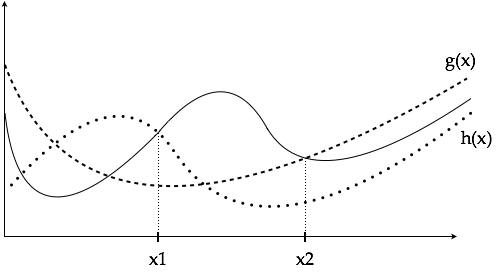
\includegraphics[scale=0.4]{FiguresArithmetic/NotationAsymptotic}
\caption{Plots of three functions: $f$ (solid curve), $f_1$ (dotted
  curve that starts out above $f$, and $f_2$ (dotted curve that starts
  out below $f$).  Assume that the three illustrated trajectories
  continue in the indicated relationships for all $x > x_2$---i.e.,
  with the plot for $f$ strictly below that for $f_1$ and strictly above
  that for $f_2$.  With this assumption, the figure illustrates the
  relations: $f_1(x) = \Omega(f(x))$ and $f_2(x) = O(f(x))$.}
\label{fig:Asymptotic}
\end{center}
\end{figure}
{\Denis check caption}

\ignore{*********
\subsubsection{Getting formal}

{\small\sf Big-$O$, Big-$\Omega$, and Big-$\Theta$ notation}.%
It is convenient to have terminology and a notation that allows us to
talk about the rate of growth of one function as measured by the rate
of growth of another.  We are interested in the exact growth rate, as
well as upper and lower bounds on the growth rate.  We do have
appropriate such language for certain rates of growth.  We can talk,
for instance, about a linear growth rate or a quadratic rate or an
exponential rate, to name just a few---and we get the desired bounds
using the prefixes ``sub'' or ``super,'' as in ``subexponential'' and
``superlinear''---but our repertoire of such terms is quite limited.
Mathematicians working in the theory of numbers in the late nineteenth
century established a notation that gives us an unlimited repertoire
of descriptors for growth rates, via what has come to be called the
big-$O$, big-$\Omega$, and big-$\Theta$ notations, which are
collectively sometimes called {\em asymptotic notation}.\index{asymptotic notation}
*******}

\subsection{The ``Uncertainties'' in Asymptotic Relationships}
\label{sec:uncertainties-asymptotics}

The formal definitions of all three of our asymptotic relationships
are bracketed by two important quantifiers:
\[ ``(\exists c >0)'' \ \ \ \mbox{ and } 
 ``(\forall x > x^{\#})''.
\]
The former, {\em uncertain-size} quantifier, asserts that asymptotic
notions describe functional behavior ``in the large''.  Thus, in
common with more common qualitative descriptors of quantitative growth
such as linear, quadratic, cubic, quartic, exponential, logarithmic,
etc., asymptotic relationships give no infomation about constants of
proportionality.  {\em We are not saying that constant factors do not
  matter!  We are, rather, saying that we want to discuss growth
  patterns \underline{in the large}.}

The latter, {\em uncertain-time} quantifier asserts that asymptotic
relationships between functions are promised to hold only
``eventually'', i.e., ``for sufficiently large values of the argument
$x$''.  Therefore, in particular, asymptotic notions cannot be
employed to discuss or analyze quantities that can never grow beyond a
fixed finite value.  The fact that all instances of a quantity
throughout history have been below $N$ is immaterial, as long as it is
conceivable that an instance larger than $N$ could appear at some time
in the future.

These quantifiers in particular distinguishes claims of asymptotic
relationship from the more familiar definite inequalities such as
``$f(x) \leq g(x)$'' or $f(x) \geq 7 \cdot g(x)$.  In fact, it is
often easier to think about our three asymptotic bounding assertions
as establishing {\em envelopes} for $f(x)$:
\begin{itemize}
\item
Say that $f(x) = O(g(x))$.  If one draws the graphs of the functions
$f(x)$ and $c \cdot g(x)$, then as one traces the graphs with
increasing values of $x$, one eventually reaches a point $x^{\#}$
beyond which the graph of $f(x)$ never enters the territory {\em
  above} the graph of $c \cdot g(x)$.
\item
Say that $f(x) = \Omega(g(x))$.  This situation is the up-down mirror
image of the preceding one: just replace the highlighted ``{\em
above}'' with ``{\em below}.''
\item
Say that $f(x) = \Theta(g(x))$.  We now have a two-sided envelope:
beyond $x^{\#}$, the graph of $f(x)$ never enters the territory {\em
  above} the graph of $c_1 \cdot g(x)$ and never enters the territory
{\em below} the graph of $c_2 \cdot g(x)$.
\end{itemize}
In addition to allowing one to make familiar growth-rate comparisons
such as ``$n^{14} = O(n^{15})$'' and ``$1.001^n = \Omega(n^{1000})$,''
we can now also make assertions such as ``$\sin x = \Theta(1)$,''
which are much clumsier to explain in words.

\medskip

\noindent {\bf Beyond the big letters.}\index{asymptotics!with little letters}
%
There are ``little''-letter analogues of the preceding ``big''-letter
asymptotic notations: $o$, $\omega$, and $\theta$.  The definition and
range of application of these notations build on the notion of {\it
  limit}, which is basic in continuous mathematics---e.g., in the
calculus---but rare in discrete mathematics.  We therefore do not
include this topic in this text, instead referring the reader to any
good text on the calculus.

\subsection{Inescapable Complications}
\label{sec:asymptotic-complication}

The story we have told thus far is more or less standard fare in
courses on discrete mathematics and algorithms.  Two complications to
the story are covered less consistently, although lacking them, one
cannot perform cogent asymptotic reasoning about modern computing
environments.  Both complications involve the notion of {\em
  uniformity}. \index{relations!uniformity}

\noindent
{\bf 1.}\index{asymptotics!multiple functions}
{\em Multiple functions}.
%
Say that we have four functions, $f, g, h, k$, and we know that both
\[ f(n) = O(g(n)) \ \ \mbox{ and } \ \ h(n) = O(k(n)) \]
It is intuitive that
\[ f(n) + h(n) = O(g(n) + k(n)) \]
--- but is it true?

In short, the answer is YES, but verifying that requires a bit of
subtlety, because, absent hitherto undisclosed information, the
proportionality constants $c_{f,g}$ and $N_{f,g}$ that witness the
big-$O$ relationship between functions $f$ and $g$ have no connection
with the constants, $c_{h,k}, N_{h,k}$ that witness the analogous
relationship between functions $h$ and $k$.  Therefore, in order to
verify the posited relationship between functions $f + h$ and $g + k$,
one much find witnessing constants $c_{f+h, g+k}$ and $N_{f+h,g+k}$.
Of course, this task requires only elementary reasoning and
manipulation --- but it must be done!


\noindent {\bf 2.}\index{asymptotics!multivariate functions}
{\em Multivariate functions}.
%
Finally, we discuss the scenario that almost automatically accompanies
the transition from a focus on sequential, single-agent computing to a
focus on PDC.  Within this broadened context, most functions that
describe a system have one or more variables that describe the
computing system --- its number of processors or of agents or the
sizes of its memory modules or the communication-radii of its
transponders or \ldots, in addition to the one or more variables that
describe the data that the system is processing.  Within such
scenarios, every assertion of an asymptotic relationship, of the form
\[ f(\vec{m}; \vec{n}) = O(g(\vec{m}; \vec{n})) \]
must explicitly specify the following information:
\begin{itemize}
\item
which variables can grow without bound;
\item
among such unbounded variables, which participate in the posited
asymptotic relation;
\item
for each participating unbounded variable $x$, what are the constants
$c_x$ and $N_x$ that witness the posited asymptotic relationship(s).
\end{itemize}

Clearly the complexity of cogent asymptotic reasoning --- hence also
the complexity of teaching about such reasoning --- gets much more
complicated in the multivariate settings engendered by PDC.  But, the
benefits of being able to reason qualitatively about the quantitative
aspects of computing increase at least commensurately!

\section{Reasoning about Infinity}
\label{sec:reasoning-infinity}

\subsection{Coping with infinity}
\label{sec:coping-infinity}

A recurring challenge when one ``does'' mathematics is dealing with
{\em infinity}.  Infinite objects, such as sets and summations, behave
rather differently from the more familiar finite objects that we
encounter in our daily lives.  Two examples will suffice.  
\begin{enumerate}
\item
We all know that there are ``equally many'' integers with the set of
odd integers as there are integers within the set $\N$ of all
integers.  We verify this easily by matching the two sets element by
element.  We never run out of elements of either set---even though the
first of these sets is obtained from the second by discarding half of
its elements.
\item
We have seen in Chapter~\ref{ch:Summation} that there exist summations
of infinitely many positive numbers whose sum is finite, and there
exist other such summations whose ``sum is infinite'' (in a sense that
can be made precise).  One instance of the former class of summations is:
\[ 1 \ + \ {1 \over 2} \ + \ {1 \over 2^2} \ + \cdots + \ {1 \over
  2^k} \ + \cdots \ \ = \ \ 2;
\]
in this example, the summation of the infinite set of inverse powers
of $2$ {\em converges} to the finite sum $2$; see
Proposition~\ref{thm:sum-finite-geometric-series}.  One instance of
the latter class of summations is:
\[ 1 \ + \ {1 \over 2} \ + \ {1 \over 3} \ + \cdots + \ {1 \over k} \ + \cdots; \]
in this example, the summation of the infinite set of reciprocals of
positive integers {\em diverges:} its sum increases forever as more
reciprocals are added in; see the treatment of this series in
Section~\ref{sec:riemann-bounds}.
\end{enumerate}

A more subtle challenge when dealing with the world of the infinite
manifests itself in the myriad {\em paradoxes} that one encounters in
this world.  Does an arrow ever reach its target---given that it
begins its journey by traversing half then distance, then traverses
half of the remaining half, then half of the remaining quarter,
\ldots?

\ignore{*********
{\Denis This part should be carefully read}

{\Arny An immediate problem is the forward reference to SUMMATION.  Do
  we need to reorganize?}

We presented in the chapter Summations several ways to compute the sum
of numbers in a given sequence ($a_n$).  If the sequence contains
infinitely many, the sum can be finite or not.  Some of the classical
techniques used while calculating finite sums are no longer valid for
infinite sums.


A natural definition is $\sum_{k \geq 1} a_k = lim_{n \rightarrow \infty} \sum_{k=1}^{n} a_k$.
But we have to be careful with this definition. 
For instance, let us consider the following paradoxal situation:
we aim to determine the value of $S = \sum_{k \geq 0} \frac{1}{2^k}$.
Defining the infinite sum as the limit leads to the value $2$. 
This is obtained $2S = S+2$...
But what happens if we apply the same reasoning to to the sum: $\sum _{k \geq 0} 2^k$?
To obtain the value $-1$!
This is obviously not correct since the sum of increasing positive numbers should be positive.
The reason is that the terms of the series grows to $+\infty$.
**********}

\subsection{The ``Point at Infinity''}
\label{sec:point-at-infinity}

In large part, the difficulties encountered when dealing with infinite
objects result from the conceptual fiction that there is, in fact, a
``point at infinity''---i.e., that one can treat infinity as just
another number.  In many mathematical environments, this fiction is an
aid to reasoning which can be handled with totally rigor---but often
only when accompanied by rather sophisticated mathematical machinery.
Two familiar examples of such mathematical machinery are the notions
of \index{limit} {\it limit} and \index{continuity} {\it continuity}
(of a function).  A more advanced example of such machinery is the
{\it Riemann sphere}, \index{Riemann sphere} an invention of the
19th-century German mathematician Bernhard Riemann, \index{Riemann, Bernhard} 
which allows one to reason about the infinite two-dimensional plane by
``conformally'' wrapping the plane into a sphere whose ``south pole''
represents the zero-point (i.e., the origin) of the plane and whose
``north pole'' represents the ``point at infinity.''  There are many
other, less-familiar, examples of such mathematical machinery,
including advanced topics such as {\it types} in the domain of
mathematical logic.

Of course, we have alreadt dealt successfully with a number of quite
sophisticated topics related to infinity.  To cite just two examples:
\begin{enumerate}
\item
In Chapter~\ref{ch:numbers-numerals} we successfully answer questions
such as
  \begin{enumerate}
  \item
{\it Are there more rational numbers than integers?}
  \item
{\it Are there more real numbers than rational numbers?}
  \end{enumerate}

\item
In Chapters~\ref{ch:numbers-numerals} and~\ref{ch:Summation}, we
successfully summed and manipulated infinite summations.
\end{enumerate}

The lessons of the preceding paragraphs is that there is no need to
avoid dealing with infinity and its related notions---as long as one
has the mathematical machinery necessary to define all needed notions
unambiguously, obtain well-defined results from all required
operations and manipulations, and reason cogently about all concepts
and processes.  That said, the scenarios described in the following
two subsections warn us to treat all aspects of infinity with care and
respect.  The subsections point out two challenges one can encounter
when reasoning about the infinite.  Both challenges leave us with a
{\em paradox}, i.e., ``a statement or proposition that, despite sound
(or apparently sound) reasoning from acceptable premises, leads to a
conclusion that seems senseless, logically unacceptable, or
self-contradictory.''  {\small (Apple dictionary)}


\subsubsection{Underspecified problems}
\label{sec:underspecified}

The paradoxes we present now require refined groundrules for their
resolution.  The underlying problems {\em seem} to be totally
specified---until one tries to develop their solutions.

\paragraph{\small\sf A. An infinite summation}

The first question we tackle was the subject of much concern as the
topic of infinite summations emerged from its infancy in the 18th
century.  The overriding question is, What can one learn from infinite
series that do not have a unique sum?  Much valuable work was done on
this question, most being beyond the scope of this text.  But the
conundrum presented by the following, particularly vexing, infinite
summation is valuable to consider here.
\[ S \ = \ 1 \ - \ 1 \ + \ 1 \ - \ 1 \ + 1 \ - \ 1 \ + \cdots \]
There are many conflicting, but well-reasoned, answers to the following
questions.

\noindent
{\bf Questions}:  {\it Does $S$ have a finite value?  If not, then is
  $S$ positive or negative?}

\noindent
Here are three plausible answers to these questions; the third merits
some strong contemplation.
\begin{enumerate}
\item
$S \ = \ 0$

This response is justified by the following association of terms in
the summation that defines $S$.
\begin{eqnarray*}
S & = & (1 \ - \ 1) \ + \ (1 \ - \ 1) \ + (1 \ - \ 1) \ + \cdots \\
  & = & 0 \ + \ 0 \ + 0 \ + \cdots \\
  & = & 0
\end{eqnarray*}

\item
$S \ = \ 1$

This response is justified by the following association of terms in the
summation that defines $S$.
\begin{eqnarray*}
S & = & 1 \ - \ (1 \ + \ 1) \ - \ (1 \ + \ 1) \ - \ (1 \ + \ 1)
          \ + \cdots \\
  & = & 1 \ - \ (1-1) \ - \ (1-1) \ - \ (1-1) \ - \cdots \\
  & = & 1
\end{eqnarray*}

\item
There is no valid answer, because the problem statement does not
specify how to associate terms.  Indeed, by mischievously playing with
parentheses, one can arrive at many ``plausible'' values for $S$.
This is one concrete example of how summations with infinitely many
terms behave differently from those with finitely many terms.
\end{enumerate}


\paragraph{\small\sf B. The Ross-Littlewood paradox}

The following story about balls and bins is known as the {\it
  Ross-Littlewood paradox}, after its creators: A version of the story
appeared first in John Littlewood's enlightening and entertaining book
{\it Littlewood's Miscellany;} \cite{Littlewood-misc}
\index{Littlewood, John E.} the story was amplified to its present
form by S.M.~Ross \cite{Ross76}. \index{Ross, Sheldon M.}

Let us imagine a system that contains
\begin{itemize}
\item
a {\em really big} bin (in fact, one whose capacity grows as needed,
as the story progresses)
\item
an unbounded sequence of ordered balls, labelled 1, 2, \ldots
\item
a {\em very} (read: infinitely) precise clock.
\end{itemize}
The system is watched over by a {\it Keeper}.  We observe
the {\it Keeper} executing the following process.

Step $1$ of the process occurs at time {\em midnight minus $1$
  minute}.  The {\it Keeper} places the first ten balls in the
sequence (balls \#$1, \ldots, 10$) into the bin, and {\em immediately}
removes the first ball (ball \#$1$).

Step $2$ of the process occurs at time {\em midnight minus $1/2$
  minute}.  The {\it Keeper} places the next ten balls in the sequence
(balls \#$11, \ldots, 20$) into the bin, and {\em immediately} removes
the second ball (ball \#$2$).

The {\it Keeper} repeats this process endlessley, at midnight minus
$1/4$ minute (putting balls \#$21, \ldots, 30$ into the bin and
removing ball \#$3$), then at midnight minus $1/8$ minute (putting
balls \#$31, \ldots, 40$ into the bin and removing ball \#$4$), and
on, and on.

\noindent
{\bf Question}: {\it How many balls are present in the bin at
  midnight?}  (Note that ``infinity'' now measures the number of steps
executed in the process.)

\noindent
As in paragraph {\small\sf A}, there are many plausible answers to
this question.  We provide just three.
\begin{enumerate}
\item
There are infinitely many balls.

This response is justified by the following reasoning.  Each step of
the process inserts $10$ balls into the bin but removes only $1$ ball.
Hence, the population of the bin grows by $9$ balls after every step
of the process---and it never decreases!  Hence, the bin's population
after infinitely many steps must be infinite.

\item
There are $0$ balls---the bin is empty!.

This response is justified by the following reasoning.  Every ball is
eventually removed from the bin at some (finite) step of the process.
Specifically, ball \#$n$ is removed at step $n$, i.e., at time
midnight minus $2^{-n}$ seconds.

\item
There is no valid answer, because there is no ``moment at infinity''
that is encountered after an infinite number of steps of the process.
In other words, infinity is not a number!
\end{enumerate}


\paragraph{\small\sf C.  Zeno's paradox: Achilles and the tortoise}

In his celebrated {\it Paradox of Achilles and the Tortoise}, Zeno of
Elea \index{Zeno of Elea} \index{Zeno!Zeno's paradox} presented a
problem whose solution had to await the 17th century.  In the story,
the slow-footed Tortoise (T) tries to convince the speedy Achilles (A)
of the futility of trying to win any race in which A gives T even the
smallest head start.  As long as T is ahead of A, says T, every time A
traverses half the distance between himself and T, T will respond by
moving a bit further ahead.  Thereby, T will always be a positive
distance ahead of A, so that A can {\em never} catch T.  At first
glance, this story seems to call into question the physical reality of
all motion.

The resolution of the apparent paradox resides in the notion of
\index{infinitesimals} {\em infinitesimals}---quantities that
dynamically grow smaller than any finite number.  While familiar today
to anyone who has studied subjects such as the differential calculus,
the notion of infinitesimal actually dates back only a few hundred
years, to the 17th century.  Underlying the discovery/invention of
infinitesimals is one of the great real-life mysteries of all time:
Who invented/discovered infinitesimals.  The parties to this dispute
were the German mathematician Gottfried Leibniz \cite{Leibniz}
\index{Leibniz (Leibnitz), Gottfried Wilhelm} and the English polymath
(Sir) Isaac Newton \cite{Newton}.  \index{Newton, Isaac} The cases
favoring each of these great men contains enough merit to guarantee
that the dispute will likely never be settled.  We therefore list
Leibniz and Newton alphabetically and give a coarse dating of the 17th
century for the discovery.  This real-life mystery is as full of
intrigues and suspense as any that one encounters in fiction.


\paragraph{\small\sf D. Hilbert's hotel paradox}

While the final story of this section does not actually provide a
paradox, it does point out a fundamental difference between the real
world of finite capacities and an idealized world that is not so
encumbered.

Imagine that you are running a hotel that has an infinite number of
rooms which are labeled by the (entire set of) positive integers:
there is a room \#$1$, a room \#$2$, a room \#$3$, and so on.  Say
that on a particular evening, every room of the hotel is occupied by a
guest---and then a new guest arrives!

In a desire to accommodate the newcomer, you initiate the following
procedure, which was first proposed by the eminent German
mathematician David Hilbert. \index{Hilbert, David}

By means of a broadcast message to all current guests, you move each
guest who currently occupies room \#$k$ into room \#$k+1$.  Of course,
this total shift renders room \#$1$ available---so you assign this
room to the newly arrived guest.  The world is quiet once more!

Of course, this humorous story has its roots in a fundamental
distinction between the world of finite-capacity hotels that we live
in and the idealized infinite-capacity hotel proposed in Hilbert's
story.  In a word, every finite set of integers---think of the
integers as the room numbers in a finite-capacity hotel---{\em has a
  largest number}, while an infinite set of positive integers {\em
  does not have a largest number}.


\subsubsection{Foundational paradoxes}
\label{sec:paradoxes}

The ``foundational'' paradoxes that we present now can be resolved
only via the development of new, sophisticated, mathematical
machinery.

\paragraph{\small\sf A.  G\"{o}del's paradox: Self-referentiality in language}

Let us focus on the following utterance, which we call ``Sentence $S$''.

Sentence $S$: {\em The sentence you are reading at this moment is false.}

\noindent
{\bf Questions}: {\it Is Sentence $S$ true, or not?}

\noindent
Let us analyze the options.
\begin{itemize}
\item
On the one hand: \\
If Sentence $S$ is true, then one must accept its assertion that
Sentence $S$ is false.

\item
On the other hand: \\
If Sentence $S$ is false, then one must reject its assertion that
Sentence $S$ is false.  In other words, one must conclude that
Sentence $S$ is true.
\end{itemize}

\noindent
In the 1930s, the revolutionary philosopher/ logician Kurt G\"{o}del
\index{G\"{o}del, Kurt} turned the mathematical world on its head with
his demonstration that, roughly speaking,

\begin{tabular}{l}
{\em Any language that is self-referential---i.e., that can refer to
  its own sentences} \\
{\em as objects of discourse---must contain a sentence such as
  Sentence $S$, which} \\
{\em is neither true nor false.}  \cite{Goedel31}
\end{tabular}

The shocking implication of G\"{o}del's work is that in any
sufficiently sophisticated language $L$, the notions {\it true} and
{\it false} do not totally partition (into two pieces) the set of
legitimate utterances in language $L$.  The simplicity of Sentence $S$
and encodings thereof---see, e.g., \cite{Rosenberg09}---can be used to
show that the following classes of languages, and their kin, are
``sufficiently sophisticated'':
\begin{itemize}
\item
Natural languages (Swahili, German, Urdu, etc.)
\item
General-purpose programming languages (assembly language, Basic, C,
Java, LISP, Python etc.)
\item
Quantified mathematical languages---i.e., ones that contain logical
quantifiers such as {\sc for all} ($\forall$), {\sc there exist}
($\exists$), etc.
\end{itemize}

Of course, the world proceeded before G\"{o}del's earthshaking proof,
and it is still spinning after the proof.  We are just aware now that
we must be more careful in our use of language.  For instance, we must
employ pre-validated transformations in our compilers and
pre-justified ``small steps'' in our schedulers.


\paragraph{\small\sf B.  Russell's paradox: There is no ``anti-universal'' set}

The notion of set is perhaps the most primitive one in mathematics.
Even before delving into Chapter~\ref{ch:sets-BA-logic}'s survey of
the intricacies of sets and their mathematical kin, the reader
probably has at least an informal command of many of the relevant
notions.  One of the most basic features of sets is that their
elements are not governed by any {\it a priori} restrictions.  Most
specifically for our purposes here, a set can have sets as elements.
Indeed, there is no inherent reason why a set cannot contain itself as
an element!  At first blush, this possibility for self-membership
seems to be a rather innocuous freedom.  But, the 20th-century English
philosopher/logician Bertrand Russell
\index{Russell, Bertrand}
% and Alfred North Whitehead  \index{Whitehead, Alfred North}
pointed out in \cite{Russell02,Russell03} that, when encountered
within the world of potentially-infinite sets, the capacity for
self-membership is (intellectually) hazardous.

Russell had the foresight to observe that, absent any restrictions on
the formations of sets, one could talk about the following set $A$,
which we shall call ``anti-universal.''

{\em $A$ is the set of precisely those sets that {\em do not} contain themselves
  (as elements).}

\noindent
{\bf Question}.  {\it Is the set $A$ a member of itself?}

\noindent
Let us consider the possibilities.
\begin{itemize}
\item
If set $A$ is a member of itself, then by definition, $A$ {\em does
  not} contain itself---since sets belonging to $A$ {\em do not}
contain themselves.

\item
If set $A$ is not a member of itself, then by definition, $A$ is an
element of $A$.
\end{itemize}

There have been many attempts to resolve the dilemma inherent in the
preceding analysis.  Many have striven for logical edifices that
declare the question ``{\it Is the set $A$ a member of itself?}''
somehow illegitimate.  One options that appeals to many is to assign
each sentence within a language $L$ a {\it type} (say, a positive
integer).  One then allows a sentence of $L$ to refer only to
sentences of lower type-number.

The stratagem of typing utterances within a language $L$ disables
self-reference within $L$, hence defines away both Russel's paradox
and G\"{o}del's paradox.



